\typeout{NT FILE chapter2.tex}%

\chapter{Viability of an X-ray Spectrum's Effective Energy for Use in Simulation}
\label{cha:xray_tracer_validation}

\par Currently, this ray-tracing model assumes a single energy x-ray (monoenergetic) is traveling through the objects in the scene; however, with actual x-ray machines, a wide range of energies (polyenergetic) is observed. This observed spectrum has the following explanation: inside an x-ray tube, electrons build up on a filament and are accelerated to an anode as a result of a high voltage being applied across the filament (cathode) and the x-ray target (anode). As the electrons hit the target, often made of tungsten, the electrons have a low probability of being slowed down and deflected by the positive charge of the protons in the target nucleus. The kinetic energy of the electrons lost due to this attraction is converted to an electromagnetic wave of equal energy, and increases with proximity to the nucleus. This phenomenon is called \textit{bremsstrahlung radiation} and is the only source of these x-rays at kVp's below 69.5 keV. In the extremely rare case that an electron loses all of its kinetic energy due to this nucleus interaction, the maximum energy x-ray is produced and is equal to the accelerating voltage of the tube, which is referred to as the spectrum's kVp (kilovolt peak). Once a tube's kVp rises above 69.5 keV, the binding energy of tungsten's K shell, a vacancy will be left in the K shell and electrons from the L shell, which has a binding energy of 11.5 keV, will fill this vacancy, producing an x-ray of energy $69.5 - 11.5 = 57.0$ keV. As a result, as the kVp of the tube increases, intensity spikes resulting from electron transitions will appear in the x-ray energy spectrum \cite{Seibert}.

\par Therefore, to better model reality, it would be best to redesign the ray-tracing model to produce photons according to an energy distribution; however, this would involve thousands of photons per pixel, which would drastically increase the render time of the simulation. An alternative option would be to find the singular x-ray energy that would result in the same attenuation as a particular energy spectrum produced by a tube, which is called the effective energy \cite{Seibert}. With this energy, one would be able to obtain approximately the same results as the spectrum of energies produced by the x-ray machine, eliminating the need to complicate the model and increase computation time. While this effective energy technique would solve many of the simulation's problems, the factors that affect the effective energy must first be determined.

\section{Methods}
\par In particular, the following factors were tested: an object's composition, geometry (thickness), and position in the x-ray detector. To test any of these factors, one must first determine how to obtain the effective energy, $E_{\text{eff}}$, from an x-ray image. Solving Equation~\ref{eq:exp_atten} for $\mu_m$ yields the following relationship:
\begin{equation}
    \mu_m = \frac{\ln{(I_0/I)}}{\rho l}.
\label{eq:mu}
\end{equation}
\par With $\mu_m$ being a function of effective energy, one can refer to experimental data to relate a value of $\mu_m$ to its associated effective energy. Therefore, with NIST's data \cite{hubbell1982photon} and Equation~\ref{eq:mu}, one can find the $I_0$, $I$, and $l$ for a particular x-ray image and determine the effective energy of the spectrum at the set kVp.

\par To obtain these values, a small surgical x-ray machine called the GE MiniView 6800 Mini C-Arm was used in the anatomy lab at Saint Vincent College. In order to test the composition dependence of the effective energy, images were taken of aluminum (labeled N), iron, magnesium, water, and a plastic scintillator. The thickness and density of each attenuator can be found in Table~\ref{table::matTable}. Several images were taken for each object, with kVps ranging from 40 keV to 60 keV. For each image, the object was placed in the center of the imaging area of the C-Arm, and the kVp was set with the kVp controller located on the machine. Once ready, a remote was used to activate the machine, which then sent x-rays from the tube toward the imaging area. A diagram of this setup is presented in Figure~\ref{figure:CArmDiagram}.

\begin{table}[H]
	\centering
    \begin{tabular}{ccc}
	\toprule
	Attenuator           & Thickness (cm) & Density (g/cm$^3$) \\
	\midrule
	Aluminum (N)         & 0.23           & 2.7                               \\
	Aluminum (I)         & 0.081          & 2.7                               \\
	Iron                 & 0.01           & 7.87                              \\
	Magnesium            & 0.1            & 1.46                              \\
	Plastic Scintillator & 1.98           & 1.03                              \\
	Water                & 5.80           & 1.0           			\\
	\bottomrule
\end{tabular}

    \caption{The thicknesses and densities of materials used in obtaining effective energy values.}
    \label{table::matTable}
\end{table}

\begin{figure}[H]
    \centering
	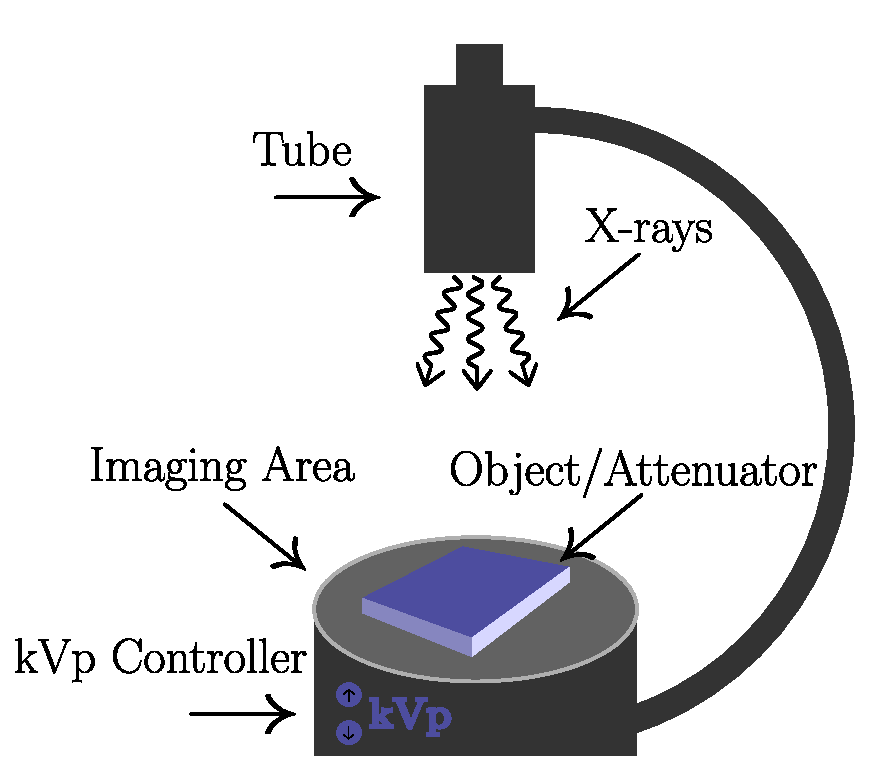
\includegraphics[scale=0.7]{chapter2/CArmDiagram.pdf}
	\caption{Diagram of GE MiniView 6800 Mini C-Arm used in effective energy measurements.}
	\label{figure:CArmDiagram}
\end{figure}

\par To test the geometrical dependence of effective energy, an image was taken of a slightly thinner sheet of aluminum (labeled I) and compared to an image of the thicker aluminum (labeled N) used for the composition experiment. Additionally, for the position dependence, an image was taken of aluminum shifted towards the edge of the imaging area. For both of these experiments, the images taken were compared to images taken at the same kVp to observe only the change in effective energy due to the factors adjusted, rather than a change due to a shift in the spectrum.

\par With images taken, $I/I_0$ had to be extracted from each image to determine $\mu_m$ using Equation~\ref{eq:mu}. For example, consider the x-ray image in Figure~\ref{figure:IntensityDiagram}: along an x-ray's journey from the tube to the detector, it encounters two different attenuators, the air and the object placed in the imaging area (with the machine setting a completely non-attenuated beam equal to 1 in the image, where 1 is white and 0 is black, the only values we can measure from pixel inspection are the relative intensities of the x-ray. Because of this, $I$ will now simply refer to the pixel intensity (0-1) and will replace $I/I_0$). In the image, $I$ becomes $I_{\text{bkg}}$ and $I_{\text{ctr}}$ for the pixel intensity in the background and center of the image, respectively. $I_{\text{bkg}}$ refers to attenuation caused by the air, while $I_{\text{ctr}}$ refers to attenuation caused by both the air and the object. Using Equation~\ref{eq:exp_atten_k}, one can show that $I_{\text{ctr}} = I_{\text{bkg}} I_{\text{obj}}$, where $I_{\text{obj}}$ is the attenuation caused by the object. Therefore, the intensity drop caused solely by the object is given by

\begin{equation}
    I_{\text{obj}} = \frac{I_{\text{ctr}}}{I_{\text{bkg}}}.
	\label{eq:IObj}
\end{equation}

\begin{figure}[H]
    \centering
	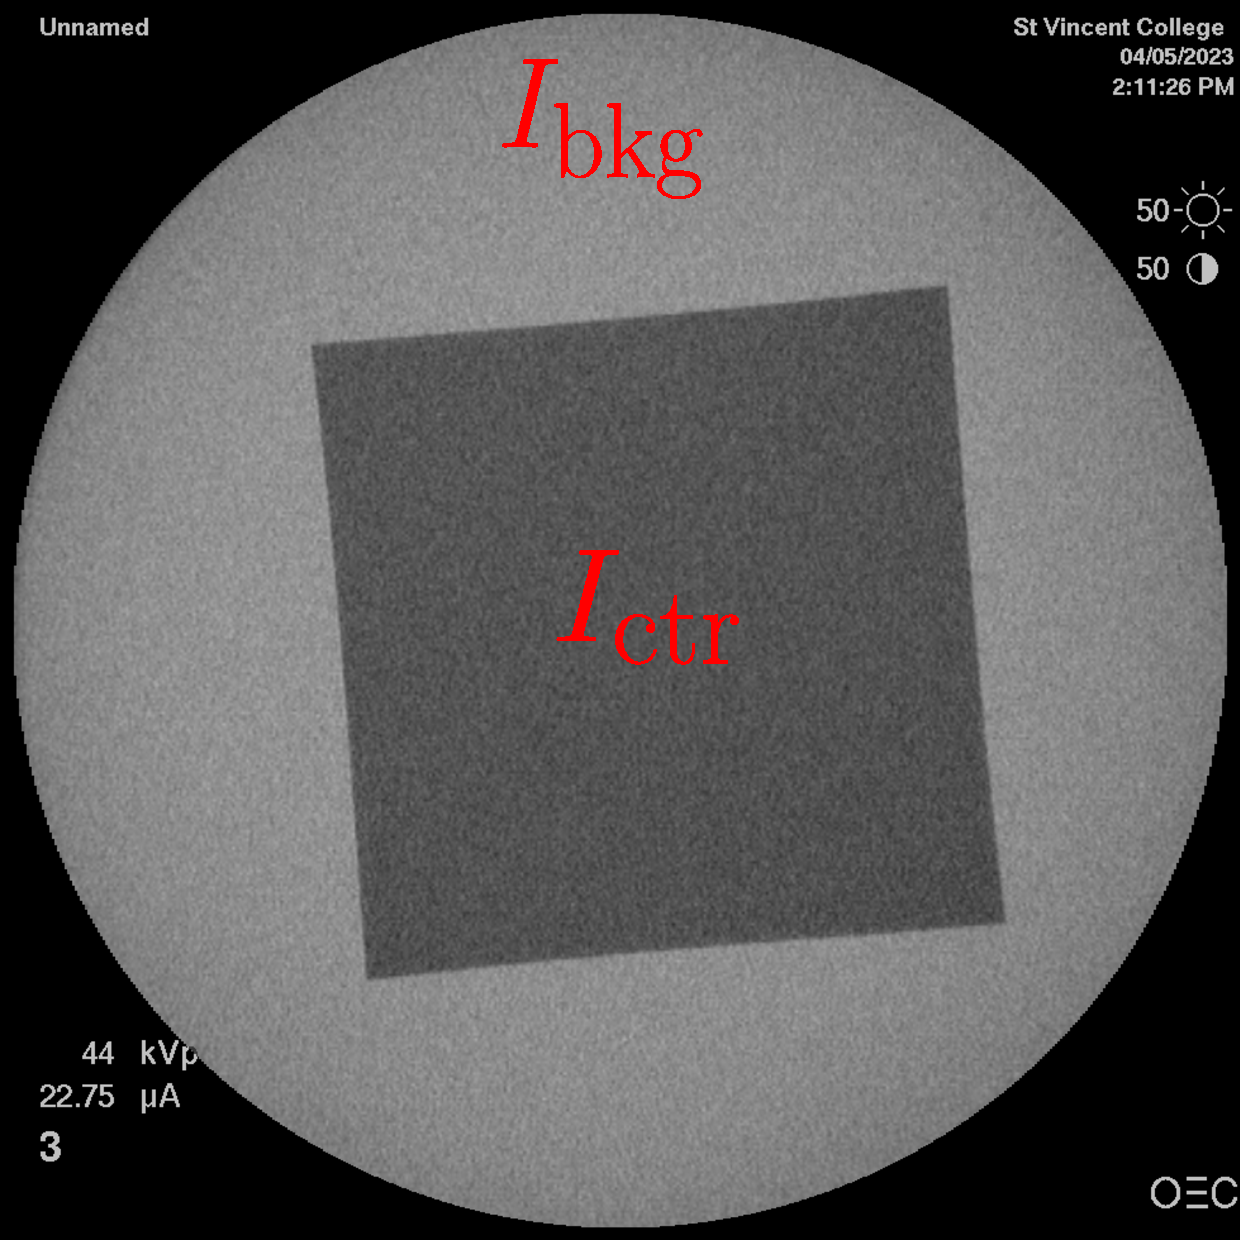
\includegraphics[scale=0.4]{chapter2/IntensityDiagram.pdf}
	\caption{X-ray image of Al at 44 kVp demonstrating the locations of the pixel values used in the calculation of $I_{\text{obj}}$.}
	\label{figure:IntensityDiagram}
\end{figure}

\par To obtain the relative intensity values in the background and center of an image, the average pixel value was taken over a square region in the desired sections of the image. With this relative intensity, extracted with the Python code in Listing~\ref{lst::extractionCode}, and the thickness of the object, the mass attenuation coefficient and effective energy of the interaction were determined using Equation~\ref{eq:mu} and NIST's database.

\begin{listing}[H]
    \begin{minted}[mathescape, linenos, numbersep=5pt, breaklines=true, fontsize=\small]{python}
        def get_relative_intensity(path, background_intensity=0):
        """
        Calculates the relative intensity of a square in the center of an image.
        :param path: Path to image
        :param background_intensity: Intensity of background
        :return: Relative intensity
        """
            # load image
            img = cv2.imread(path, 0)
        
            # convert to float and normalize
            img = img.astype(np.float32)/255
        
            # get mean pixel value and std dev 
            # of square in center of image
            center = (int(img.shape[0]/2), int(img.shape[1]/2))
            length = 100
            square = img[int(center[0]-length/2):int(center[0]+length/2), 
            int(center[1]-length/2):int(center[1]+length/2)]
        
            mean, std = cv2.meanStdDev(square)
        
            # if intensity is 1 or 0, return False,
            # so they are not used as data points
            if mean[0][0] >= 0.999 or mean[0][0] <= 0.001:
                return False
        
            # obtain relative intensity
            # by normalizing by background intensity
            # (I_square = I_background * I_object -> I_object = I_square / I_background)
            mean[0][0] = mean[0][0] / background_intensity
        
        
            # convert image to rgb
            img = cv2.cvtColor(img, cv2.COLOR_GRAY2RGB)
        
            # draw red square on image
            # and relative intensity and std on image
            cv2.rectangle(img, (int(center[0]-length/2), int(center[1]-length/2)),
            (int(center[0]+length/2), int(center[1]+length/2)), (0, 0, 255), 3)
        
            cv2.putText(img, f"Intensity: {mean[0][0]:.3f} +- {std[0][0]:.3f}", (int(center[0]-length/2),
                        int(center[1]-length/2)-10), cv2.FONT_HERSHEY_SIMPLEX, 1, (0, 0, 255), 2)
        
            return ufloat(mean[0][0], std[0][0])
    \end{minted}
    \caption{X-ray image relative intensity extraction code implemented in Python3.}
    \label{lst::extractionCode}
    \end{listing}

\section{Results}
\par To relate the calculated attenuation coefficient of a particular object to the effective energy, a $2^\text{nd}$ degree, 4 knot B-spline was used to fit NIST's mass attenuation coefficient data \cite{hubbell1982photon}. This fit, implemented with the Python package Scikit-Learn \cite{SKLearn}, provided $\mu_m = f(E_{\text{eff}})$; however, $E_{\text{eff}} = f(\mu_m)$ was needed. The described fits are shown in Figure~\ref{figure:NISTSplineFit}.


\begin{figure}[H]
    \centering
    \begin{subfigure}{\linewidth}
        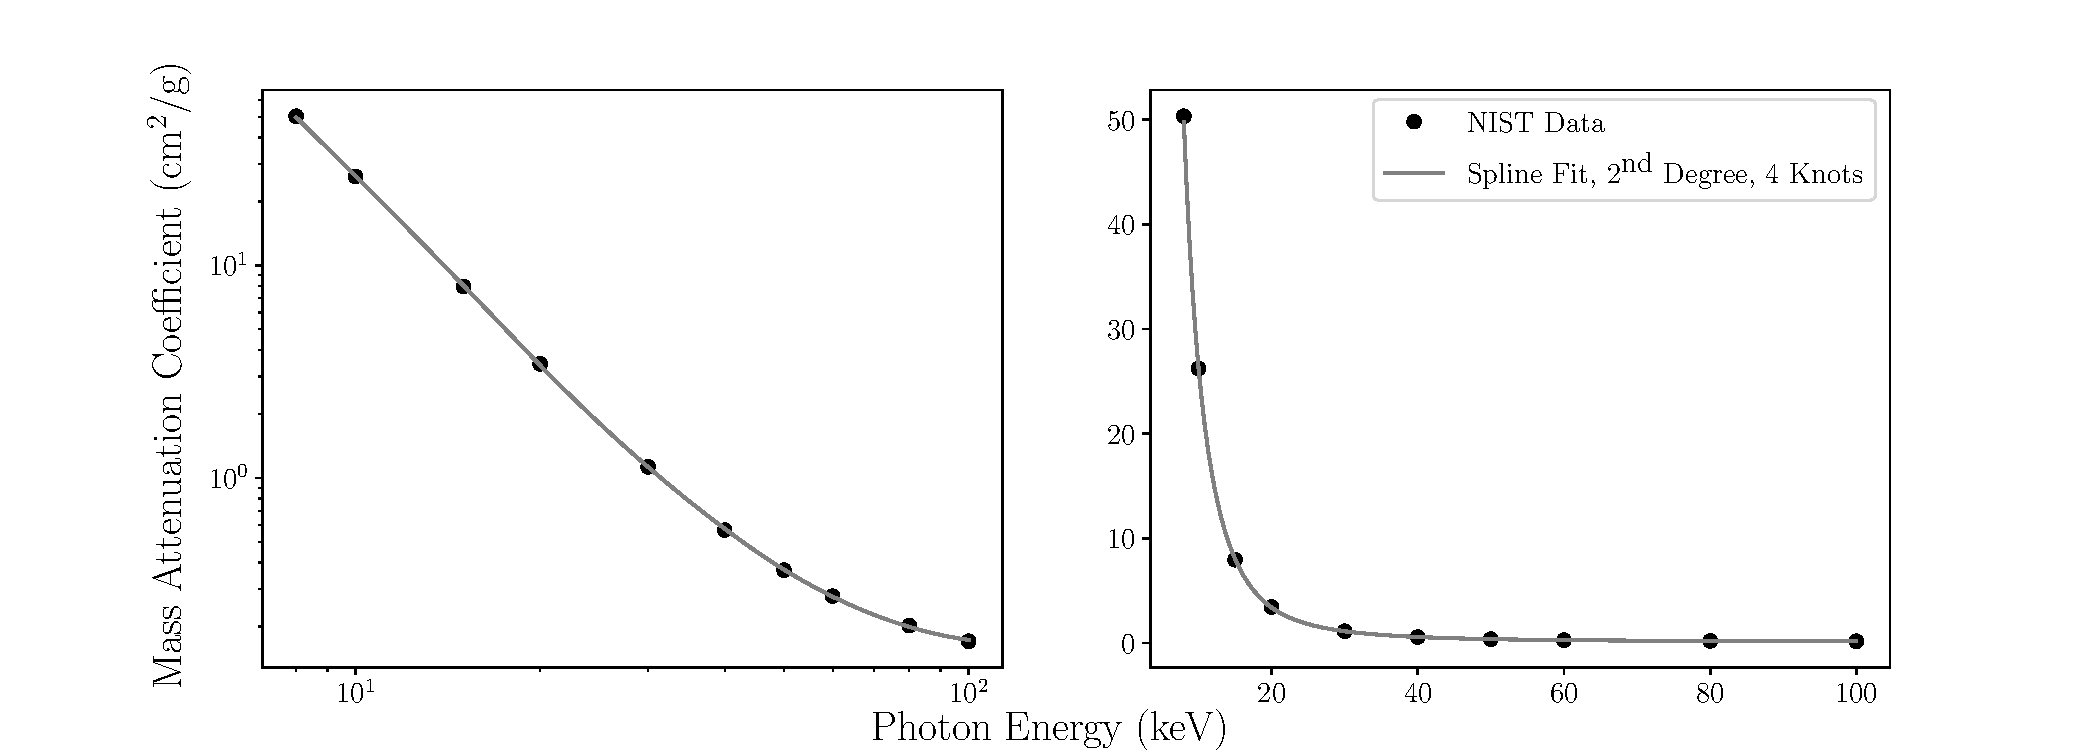
\includegraphics[width=\linewidth]{chapter2/Al_NISTSplineFit.pdf}
        \caption{Al}
    \end{subfigure}
    \begin{subfigure}{\linewidth}
        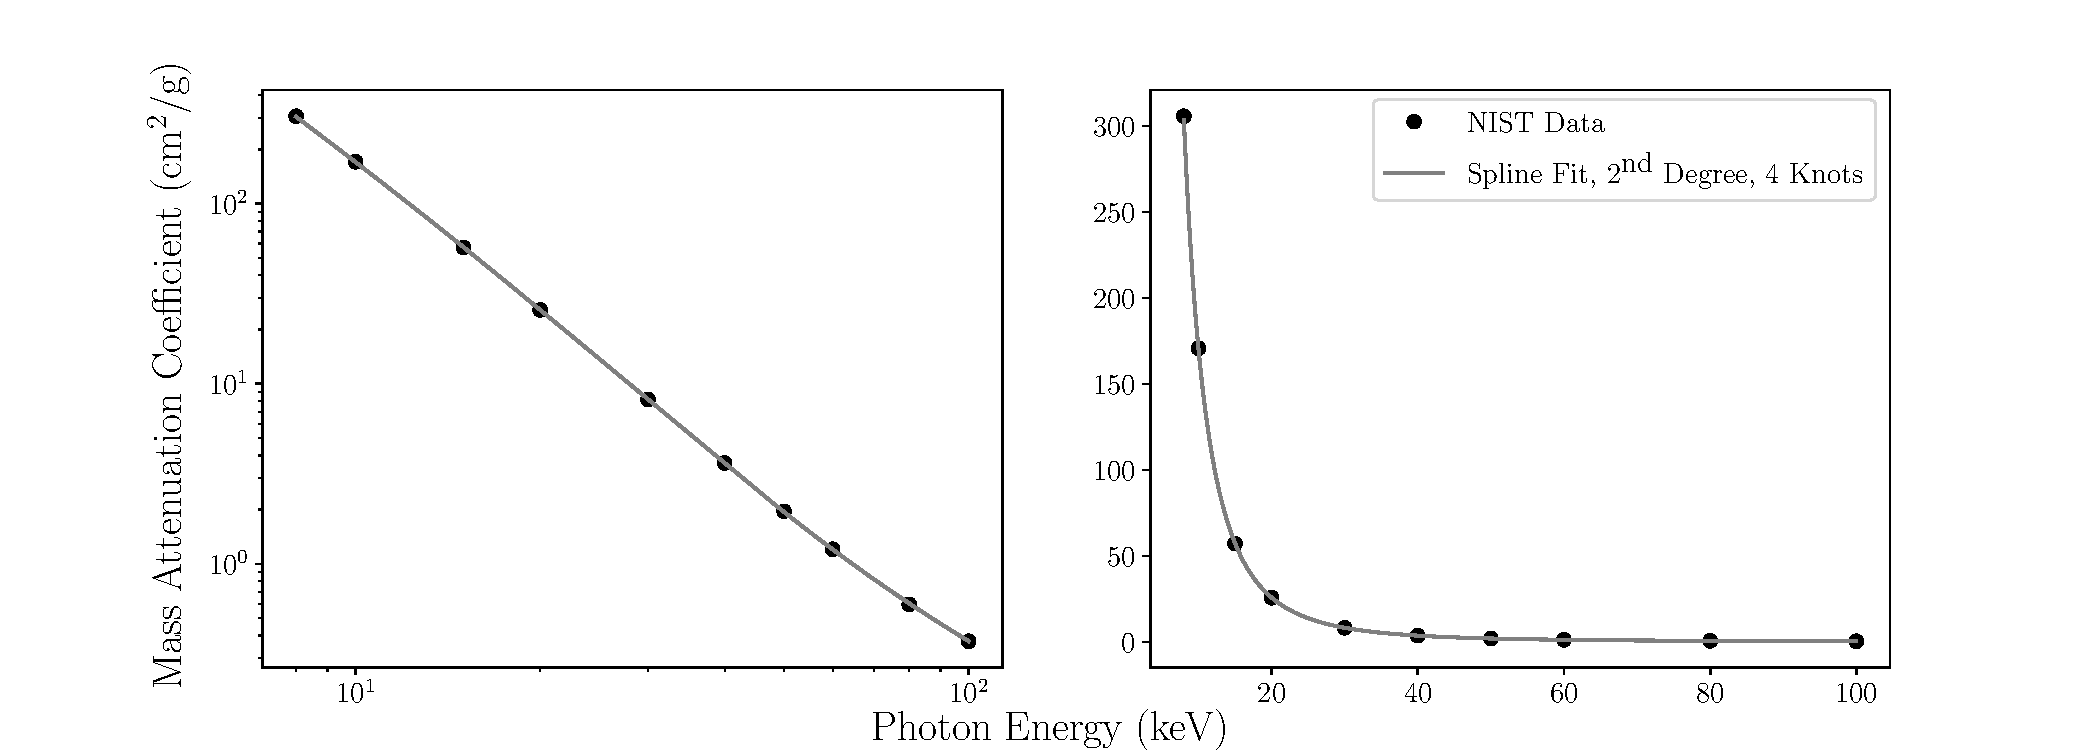
\includegraphics[width=\linewidth]{chapter2/Fe_NISTSplineFit.pdf}
        \caption{Fe}
    \end{subfigure}
    \begin{subfigure}{\linewidth}
        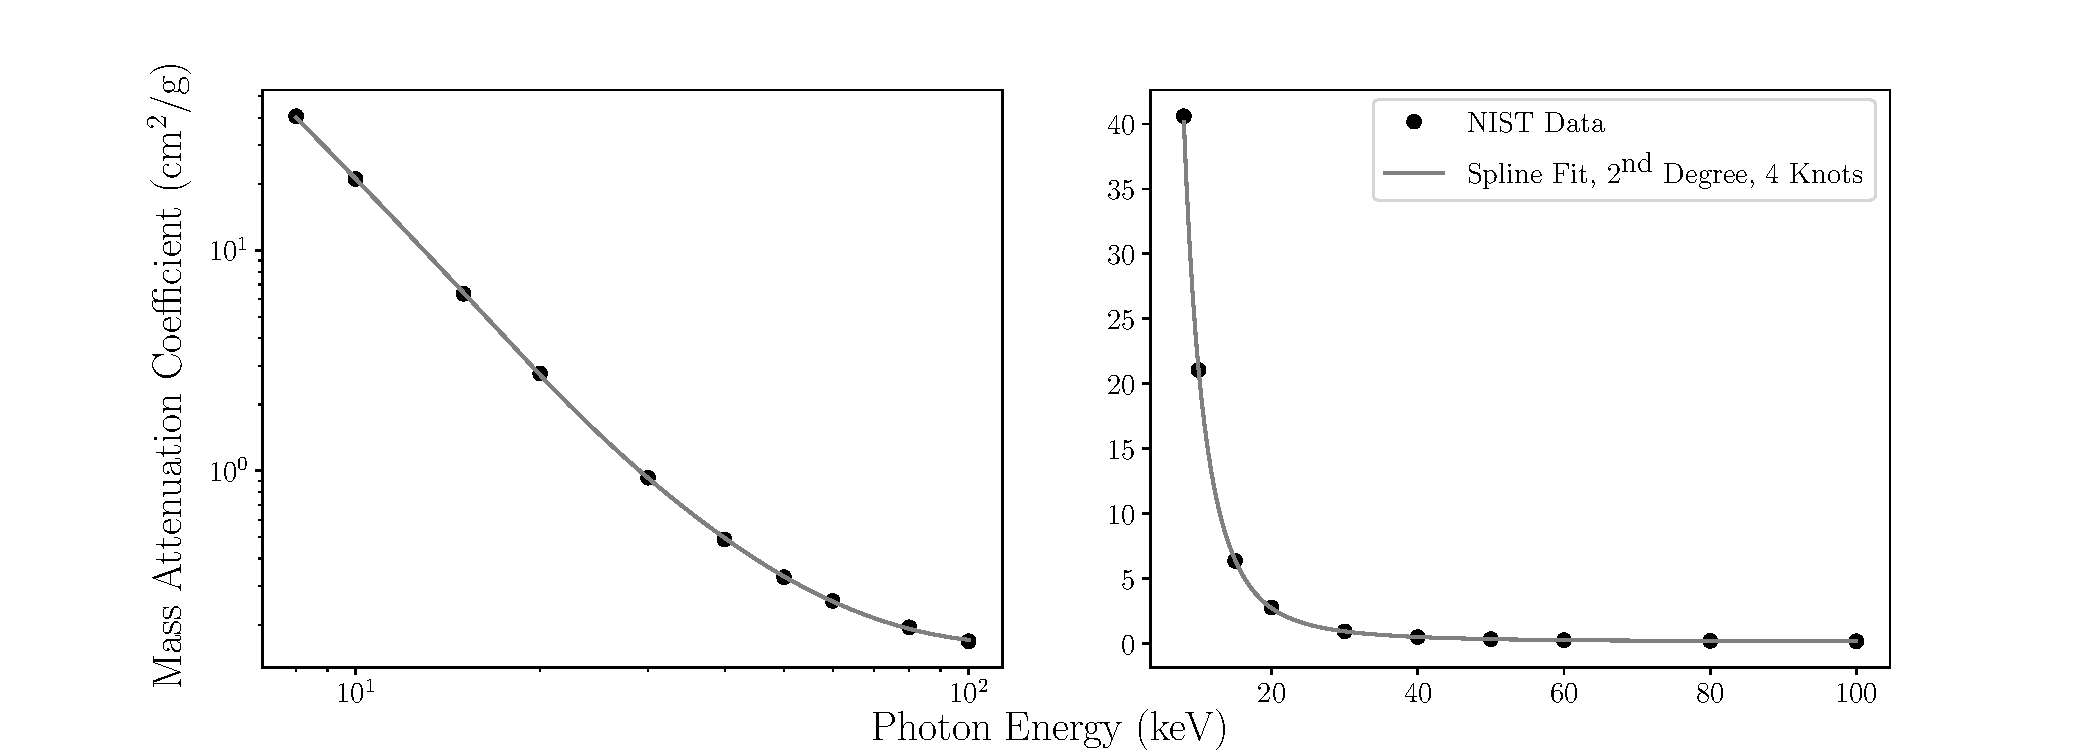
\includegraphics[width=\linewidth]{chapter2/Mg_NISTSplineFit.pdf}
        \caption{Mg}
    \end{subfigure}
\end{figure}


\begin{figure}[H]
    \ContinuedFloat
    \centering

    \begin{subfigure}{\linewidth}
        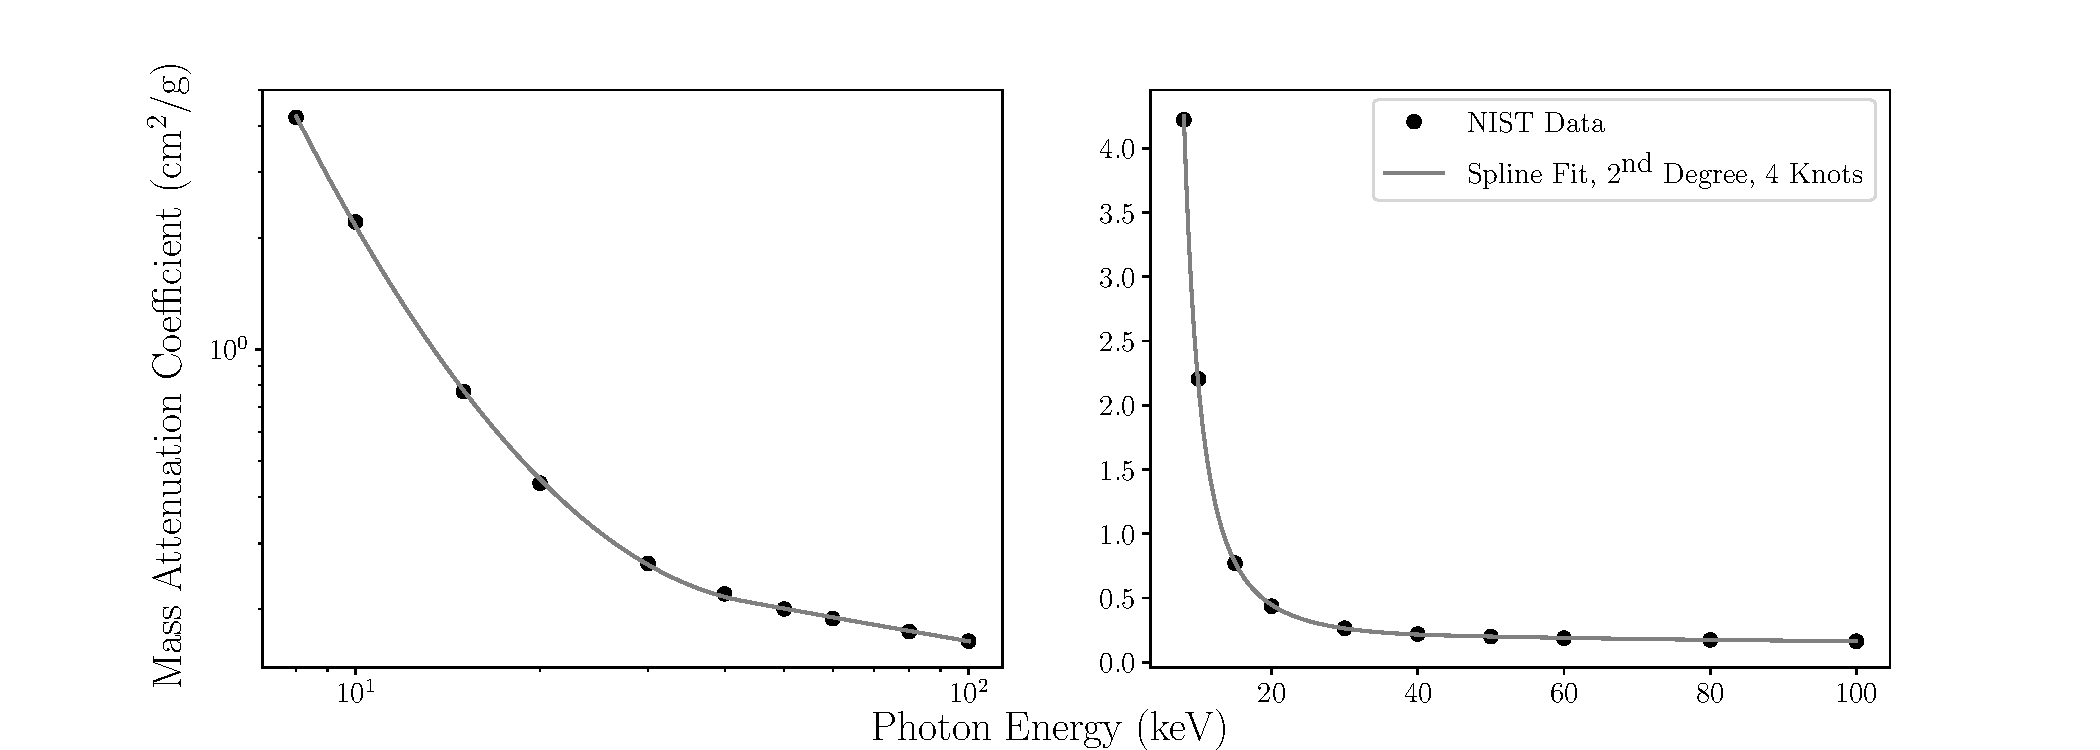
\includegraphics[width=\linewidth]{chapter2/Plastic Scintillator (Vinyltoluene-based)_NISTSplineFit.pdf}
        \caption{Plastic Scintillator}
    \end{subfigure}

    \begin{subfigure}{\linewidth}
        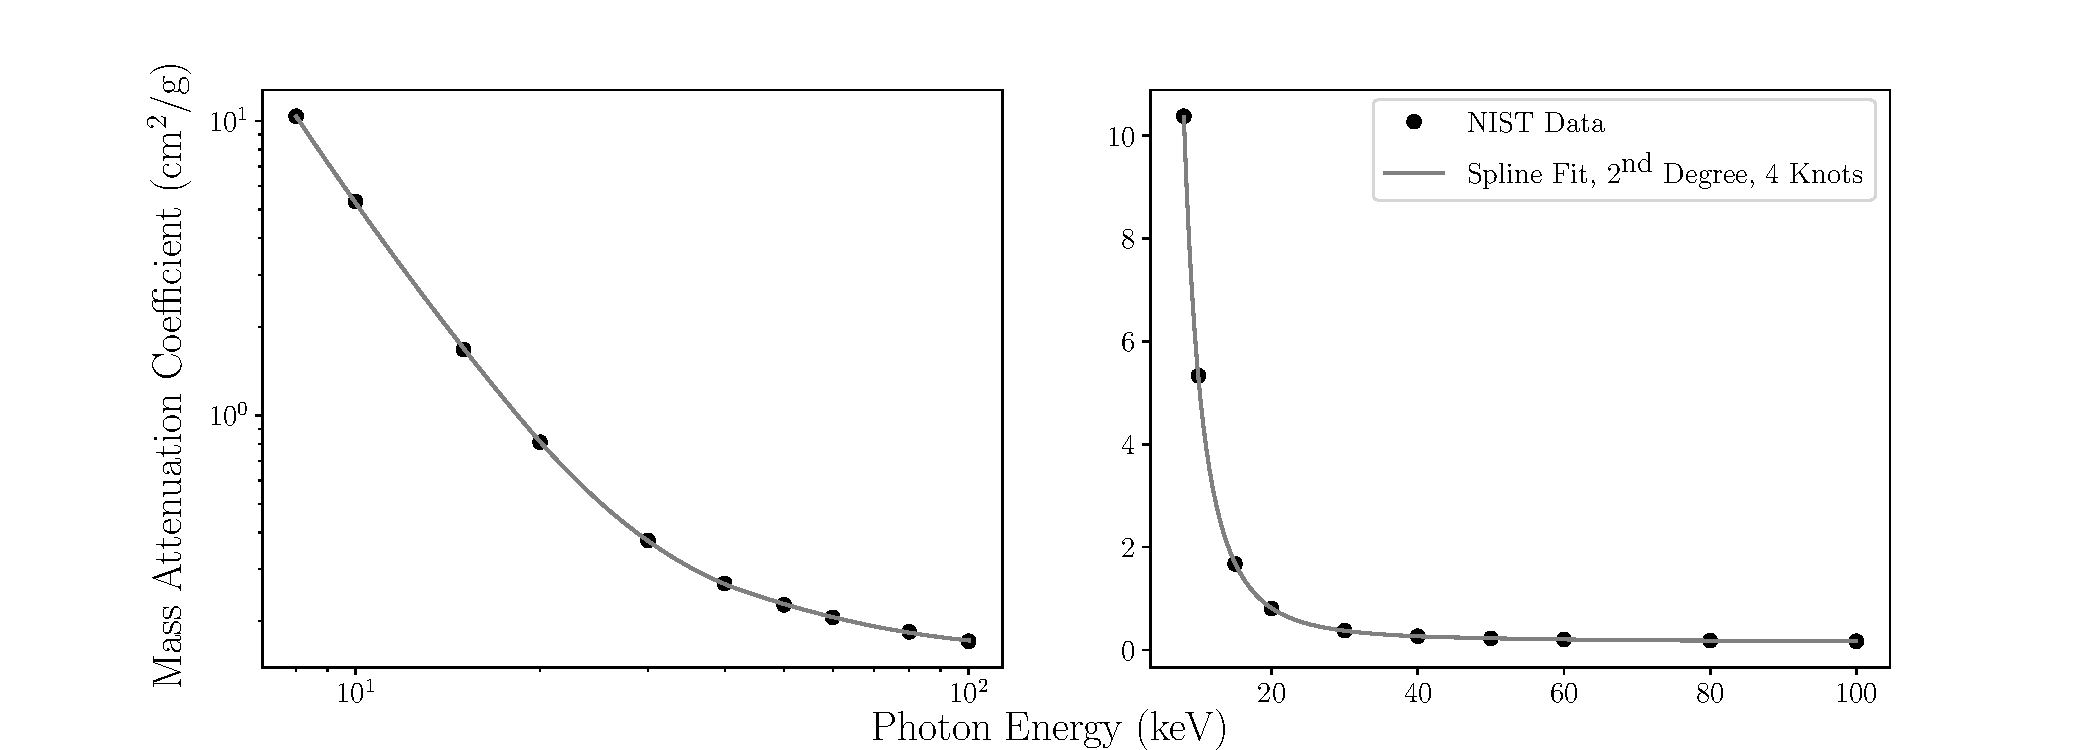
\includegraphics[width=\linewidth]{chapter2/Water, Liquid_NISTSplineFit.pdf}
        \caption{Water}
    \end{subfigure}

    \caption{The NIST mass attenuation coefficient data (in cm$^2$/g) vs. effective energy (in keV) for the Al, Fe, Mg, plastic scintillator, and water fitted using the described B-Spline. (Continued)}
    \label{figure:NISTSplineFit}
\end{figure}

\par Because $f$ represents an abstract model, an inverse was unable to be taken, so an evenly spaced $E_{\text{eff}}$ array of 10,000 values ranging from 0.8 keV to 100 keV was substituted into our model, providing its associated $\mu_m$ array. Given a particular $\mu_m \pm \sigma$, where $\sigma$ represents the sample standard deviation (Std.) of the mass attenuation coefficient, the $E_{\text{eff}}$ was found by first determining the index of the element in the $\mu_m$ array closest to the particular $\mu_m$. The associated $E_{\text{eff}}$ was then the element in the $E_{\text{eff}}$ array located at the determined index. The range of error for a particular $E_{\text{eff}}$, [$E_{\text{eff}}$ Min, $E_{\text{eff}}$ Max], was calculated by repeating the indexing process for $\mu_m + \sigma$ and $\mu_m - \sigma$. The results of this indexing technique for each X-ray image can be found in Table~\ref{table::results}.


\begin{table}[H]
    \small
    \noindent\makebox[\textwidth]{%
    \begin{tabularx}{1.27\textwidth}{ccccccccc}

    \toprule
    Material & kVp (kV) &  $I/I_0$ &  $I/I_0$ Std. &  $\mu/\rho$ (cm$^2$/g) &  $\mu/\rho$ Std. (cm$^2$/g) &  $E_{\text{eff}}$ (keV) &  $E_{\text{eff}}$ Max (keV) &  $E_{\text{eff}}$ Min (keV) \\
    \midrule
    & 40.0 &    0.310 &         0.025 &                  1.895 &                       0.131 &                  24.552 &                      25.215 &                      23.954 \\
    & 42.0 &    0.425 &         0.026 &                  1.385 &                       0.099 &                  27.635 &                      28.444 &                      26.917 \\
    Aluminum& 44.0 &    0.567 &         0.025 &                  0.920 &                       0.071 &                  32.576 &                      33.698 &                      31.591 \\
    & 46.0 &    0.668 &         0.023 &                  0.655 &                       0.056 &                  37.747 &                      39.302 &                      36.403 \\
    & 48.0 &    0.727 &         0.023 &                  0.516 &                       0.052 &                  42.145 &                      44.380 &                      40.277 \\
    & 50.0 &    0.888 &         0.020 &                  0.192 &                       0.037 &                  83.926 &                     100.000 &                      69.711 \\
    \midrule
    & 40.0 &    0.353 &         0.030 &                 13.239 &                       1.078 &                  25.316 &                      26.089 &                      24.626 \\
    & 42.0 &    0.432 &         0.031 &                 10.668 &                       0.898 &                  27.331 &                      28.196 &                      26.558 \\
    Iron& 44.0 &    0.595 &         0.030 &                  6.595 &                       0.642 &                  32.392 &                      33.588 &                      31.352 \\
    & 46.0 &    0.678 &         0.027 &                  4.937 &                       0.514 &                  35.870 &                      37.287 &                      34.646 \\
    & 48.0 &    0.761 &         0.028 &                  3.473 &                       0.461 &                  40.599 &                      42.687 &                      38.860 \\
    & 50.0 &    0.911 &         0.024 &                  1.186 &                       0.340 &                  60.335 &                      69.195 &                      54.704 \\
    \midrule
    & 40.0 &    0.632 &         0.030 &                  2.638 &                       0.274 &                  20.200 &                      20.982 &                      19.529 \\
    & 42.0 &    0.832 &         0.029 &                  1.054 &                       0.200 &                  28.444 &                      31.058 &                      26.531 \\
    Magnesium& 44.0 &    0.874 &         0.027 &                  0.776 &                       0.176 &                  32.382 &                      36.412 &                      29.668 \\
    & 46.0 &    0.909 &         0.027 &                  0.551 &                       0.172 &                  37.967 &                      46.193 &                      33.431 \\
    & 48.0 &    0.940 &         0.024 &                  0.353 &                       0.145 &                  48.162 &                      72.627 &                      39.936 \\
    \midrule
    Plastic& 40.0 &    0.578 &          0.03 &                  0.268 &                       0.025 &                  29.392 &                      32.861 &                      27.000 \\
    Scintillator& 42.0 &    0.645 &          0.03 &                  0.215 &                       0.023 &                  40.341 &                      57.906 &                      33.845 \\
    \midrule
    & 44.0 &    0.059 &         0.025 &                  0.489 &                       0.075 &                  25.500 &                      28.076 &                      23.669 \\
    Water & 46.0 &    0.220 &         0.030 &                  0.261 &                       0.024 &                  41.096 &                      46.984 &                      37.369 \\
    & 48.0 &    0.325 &         0.029 &                  0.194 &                       0.015 &                  68.652 &                      86.603 &                      58.403 \\
    \bottomrule
\end{tabularx}

    }
    \caption{The results for each non-saturated (intensities not equal to 0 or 1) X-ray image for the composition experiment.}
    \label{table::results}
\end{table}


\par The graphs of the $E_{\text{eff}}$ for each kVp and material combination can be found in Figure~\ref{figure::results}. To validate the experimental results, simulated $E_{\text{eff}}$ values were obtained with the Python module SpekPy \cite{SpekPy}, using the X-ray tube assembly specifications as provided by the manufacturer \cite{CArm}.


\begin{figure}[H]
    \centering
    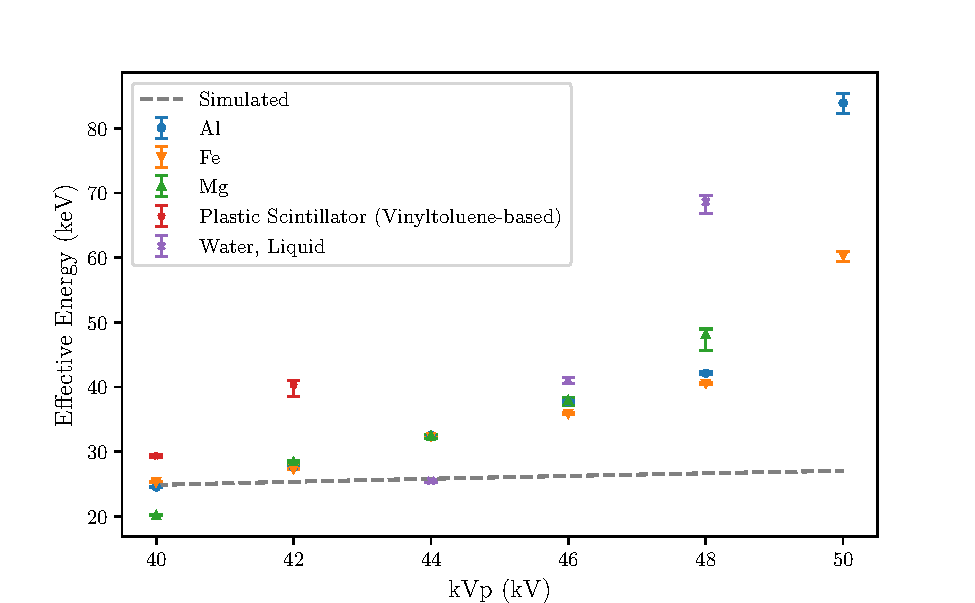
\includegraphics[width=1\linewidth]{chapter2/effEnergy.pdf}
    \caption{Graph of effective energy (in keV) vs. kVp (in kV) for the X-ray image data contained in Table (\ref{table::results}).}
    \label{figure::results}
\end{figure}

\par Figure~\ref{figure::results} shows relative agreement and an approximately linear increase for the Al, Fe, and Mg, up until 50 kVp, where a sudden spike in $E_{\text{eff}}$ is observed. For the plastic scintillator and water, vastly different values are observed. Upon further inspection by increasing the range of the fit shown in Figure~\ref{figure:NISTSplineFit}, the two values increase at an exponential rate. Furthermore, the rate of increase of $E_{\text{eff}}$ with respect to kVp is greater for the monoatomic attenuators in the experiment compared to their simulated values.

\par For the offset experiment, the intensity values for the image with the centered Al (labeled N) were obtained with the extraction code shown in Listing~\ref{lst::extractionCode}. On the other hand, the intensity values for the image with the offset Al were obtained manually using the software ImageJ. \cite{ImageJ}. The results of this experiment can be found in Table~\ref{table::offset}.


\begin{table}[H]
    \small
    \noindent\makebox[\textwidth]{%
    \begin{tabularx}{1.15\textwidth}{cccccccc}
    \toprule
    Position & $I/I_0$ &  $I/I_0$ Std. &  $\mu/\rho$ (cm$^2$/g) &  $\mu/\rho$ Std. (cm$^2$/g) &  $E_{\text{eff}}$ (keV) &  $E_{\text{eff}}$ Max (keV) &  $E_{\text{eff}}$ Min (keV) \\
    \midrule
    Center   &  0.310   &   0.025       &   1.90                &   0.13                        &   24.55                &  25.21                       &   24.00 \\
    Offset   &  0.14    &   0.05        &   3.2                 &   0.5                         &   20.5                 &  21.9                        &   19.4  \\
    \bottomrule
\end{tabularx}               

    }
    \caption{The results of X-ray images of a centered and offset Al (labeled N) at 40 kVp for use in the offset experiment.}
    \label{table::offset}
\end{table}

\par The results of this experiment show unexpected discrepancies between the centered and offset Al. A slight difference in $E_{\text{eff}}$ is expected due to the point-like nature of the x-ray source; however, it can not explain the statistical inequivalency observed due to the large distance (44.95 cm)\cite{CArm} between the x-ray source and detector; therefore, demonstrating a dependence on the object's position in the imaging area for the $E_{\text{eff}}$.

\par For the thickness-varying experiment, x-ray images of Al were taken at 40 kVp. The thickness of the Al was varied by using two different attenuators, one of thickness 2.286 mm (labeled N) and the other of thickness 0.813 mm (labeled I), as found in Table~\ref{table::matTable}. The intensity values for each image were obtained with the code in Listing~\ref{lst::extractionCode}. The results of this experiment can be found in Table~\ref{table::thickness}.

\begin{table}[H]
    \small
    \noindent\makebox[\textwidth]{%
    \begin{tabularx}{1.2\textwidth}{cccccccc}
    \toprule
    Thickness (mm) & $I/I_0$ &  $I/I_0$ Std. &  $\mu/\rho$ (cm$^2$/g) &  $\mu/\rho$ Std. (cm$^2$/g) &  $E_{\text{eff}}$ (keV) &  $E_{\text{eff}}$ Max (keV) &  $E_{\text{eff}}$ Min (keV) \\
    \midrule
    2.286          & 0.310   &  0.025        &  1.90                  &     0.13                    &   24.55                 &     25.21                   &   24.00   \\
    0.813          & 0.575   &  0.029        &  2.52                  &     0.23                    &   22.15                 &     22.92                   &   21.39   \\
    \bottomrule
\end{tabularx}

    }
    \caption{The results of X-ray images of Al (labeled N) and Al (labeled I) at 40 kVp for use in the thickness-varying experiment.}
   	\label{table::thickness}
\end{table}

\par The results of this experiment, once again, show unexpected discrepancies in $E_{\text{eff}}$ between the two thicknesses. While the $E_{\text{eff}}$'s are closer than what was measured for the offset experiment, the two values are statistically inequivalent; therefore, demonstrating a thickness dependence of the $E_{\text{eff}}$.

\section{Discussion}

\par The discrepancies between $E_{\text{eff}}$ for the monoatomic materials and the compounds have been explored extensively with little resolution. Several different theories have been explored, including the thickness of the sample, possible code errors, and the normalization of the image.

\par Upon looking for differences between the compounds and monoatomic materials, it was observed that both the compounds had a significantly larger thickness than the monoatomics, as seen in Table~\ref{table::matTable}. It was then considered whether or not the increased height of the sample could lead to an increased probability of x-rays scattering off the object and onto the detector. This effect would result in a seemingly larger background and could lead to unexpected $E_{\text{eff}}$ values. Upon manual examination of the images, the background was affected; however, the difference in intensity was minor and could not reasonably result in the exponential increase that was measured, especially since the discrepancies are still present in images where the background is non-existent.

\par Furthermore, since weighted averages of monoatomic attenuation coefficients were taken in the data processing code to obtain the attenuation coefficients for the compounds, it was considered whether or not a possible error was present in the code that could lead to this exponential behavior. Upon careful examination of the code, no errors were found, and for extra reassurance, a few images of the compounds were manually inspected, and verified the processing code's results.

\par Additionally, it was found that \textit{Heine \& Thomas} (2008) \cite{Heine} performed a similar $E_{\text{eff}}$ calibration using a mammography system. While their overall technique was similar to the methodology of this experiment, one key difference was the normalization factor used in the processing of the intensity data. In particular, they normalized the pixel value by $mAs$, which is the tube current multiplied by the exposure time. This effectively would be the incident intensity of the x-rays and is equivalent to $I_0$. However, this normalization was not able to be done for this experiment, since the C-arm does not provide any data on the exposure time for images. Still, this normalization would be the same for each kVp; therefore, this cannot explain the drastic differences between the $E_{\text{eff}}$'s of the monoatomic and compound materials that were measured at higher kVps. On the other hand, since the current of the tube was provided for each image and increased at a rate proportional to the kVp, this could explain why the $E_{\text{eff}}$'s of the monoatomic materials increased at a rate greater than what was predicted by the simulation. 

\par Finally, combining these results with the unexpected differences in $E_{\text{eff}}$ that were measured in the offset and varied thickness experiments, it is possible the x-ray machine may be doing some sort of post-processing of the images that are not described in the manual \cite{CArm}. Without knowing the specifics of this processing, the original, unfiltered images can not be calculated. Overall, the measurements obtained from this experiment reveal that the $E_{\text{eff}}$ approach for ray-tracing cannot be used for the GE MiniView 6800 Mini C-Arm. 






